Now, we can compare the results from the previous section to a non-autonomous system of ODEs, where the growth rate is a function of time, shown below.
\begin{equation}\label{eq:Non-AutonomousSystemODEs}
    \begin{aligned}
    \frac{dx}{dt} &=G(t)x\left(1-\frac{x}{K_x}\right) - c_{xy}xy,\\[.4cm]
    \frac{dy}{dt} &=r_yy\left(1-\frac{y}{K_y}\right) + c_{yx}xy.
    \end{aligned}
\end{equation}
Now, using the same parameters for the autonomous model, \equationautorefname~\eqref{eq:AutonomousSystemODEs}, we consider the model with different initial conditions.
\begin{figure}[H]
    \centering
    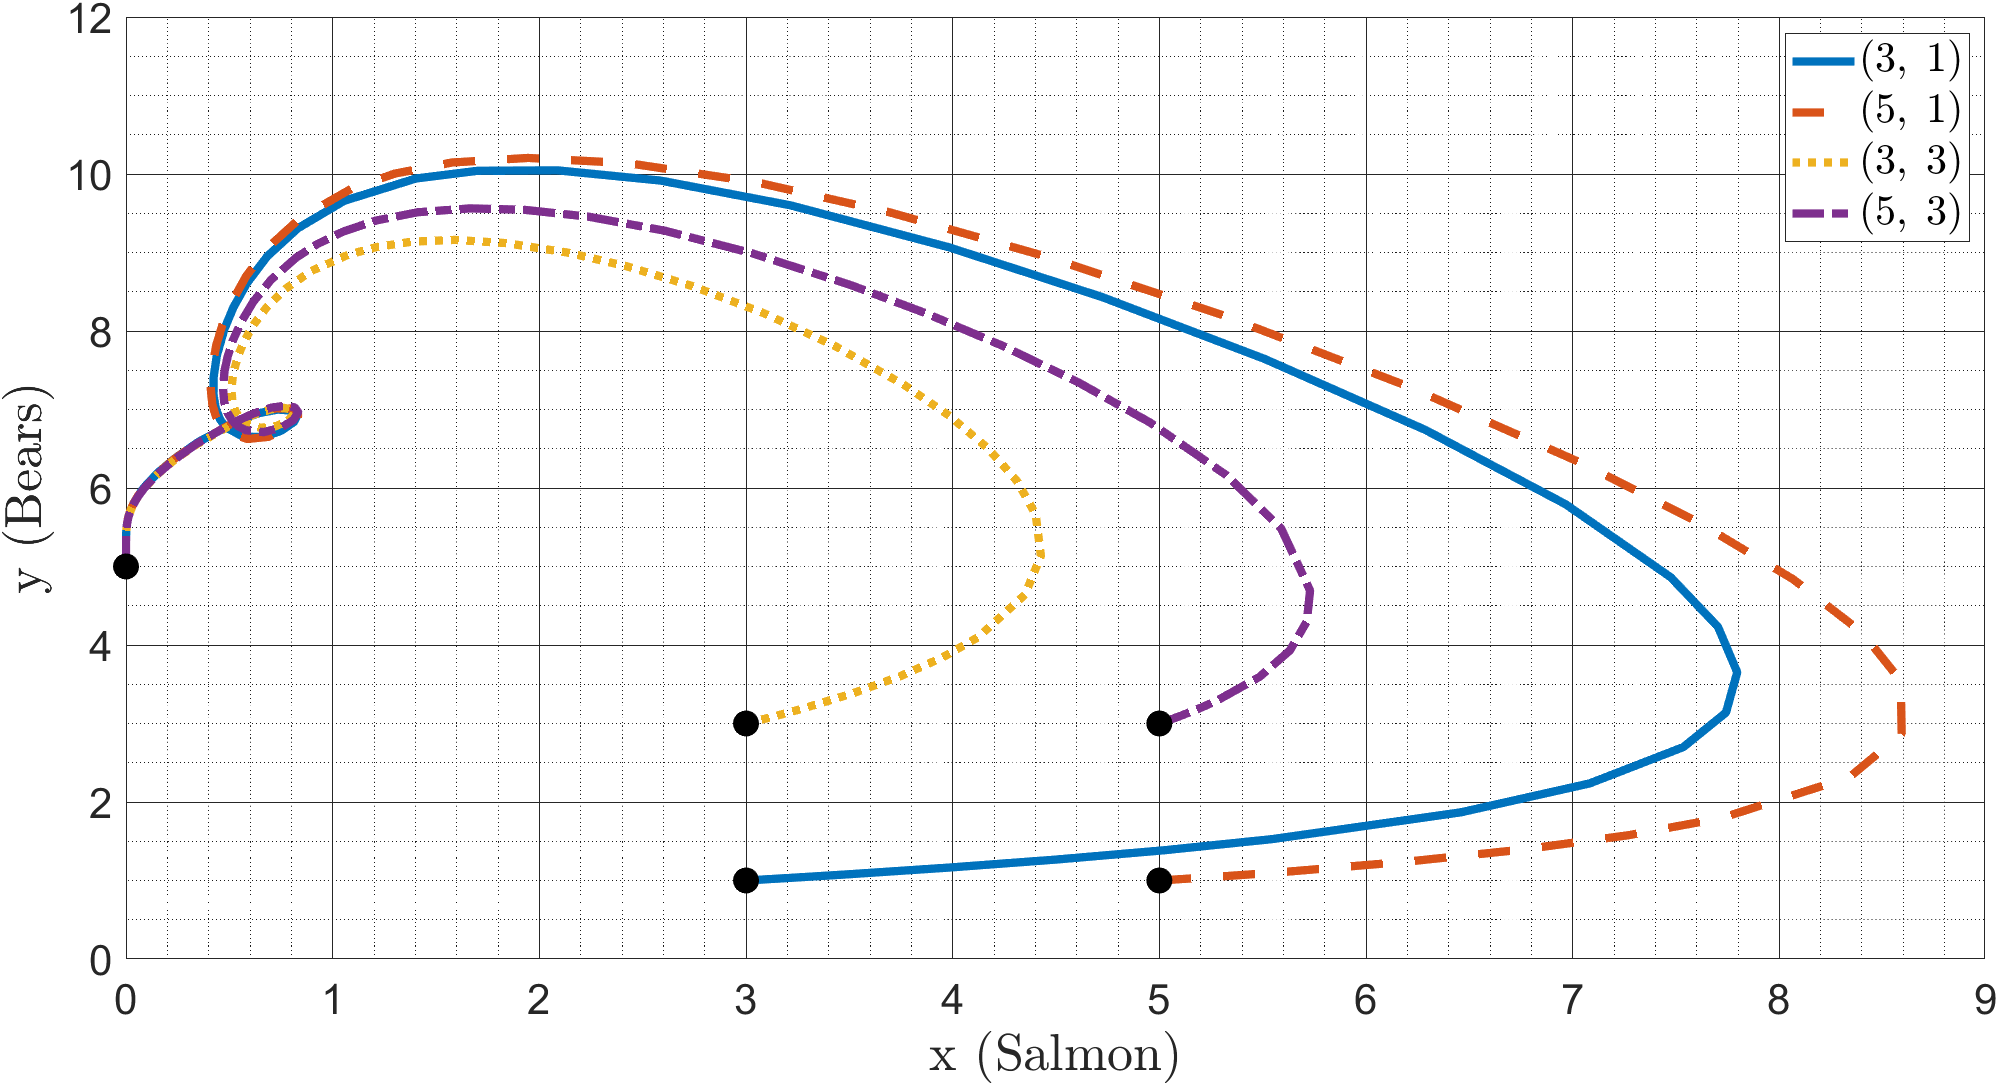
\includegraphics[width=14cm]{Pictures/Stability/SolutionsNonAutonomousModel.png}
    \caption{\singlespacing
    Compares the solutions to the non-autonomous model, \equationautorefname~\eqref{eq:Non-AutonomousSystemODEs}, with different initial conditions, $(x_0,\ y_0)$.}
    \label{fig:Non-AutonomousSystemODEs}
\end{figure}
As expected, the salmon population converges to zero as seen in \figureautorefname~\ref{fig:SalmonWithRepoFun}, resulting in the brown bear population converging to their carry capacity.
When the salmon population dies off, the interaction terms in the model will approach zero, and eventually, the behavior of the brown bear species will be represented by its logistic equation, \equationautorefname~\eqref{eq:LogBear}.
Lastly, in the graph below, we compare the results to the autonomous and non-autonomous models.
\begin{figure}[H]
    \centering
    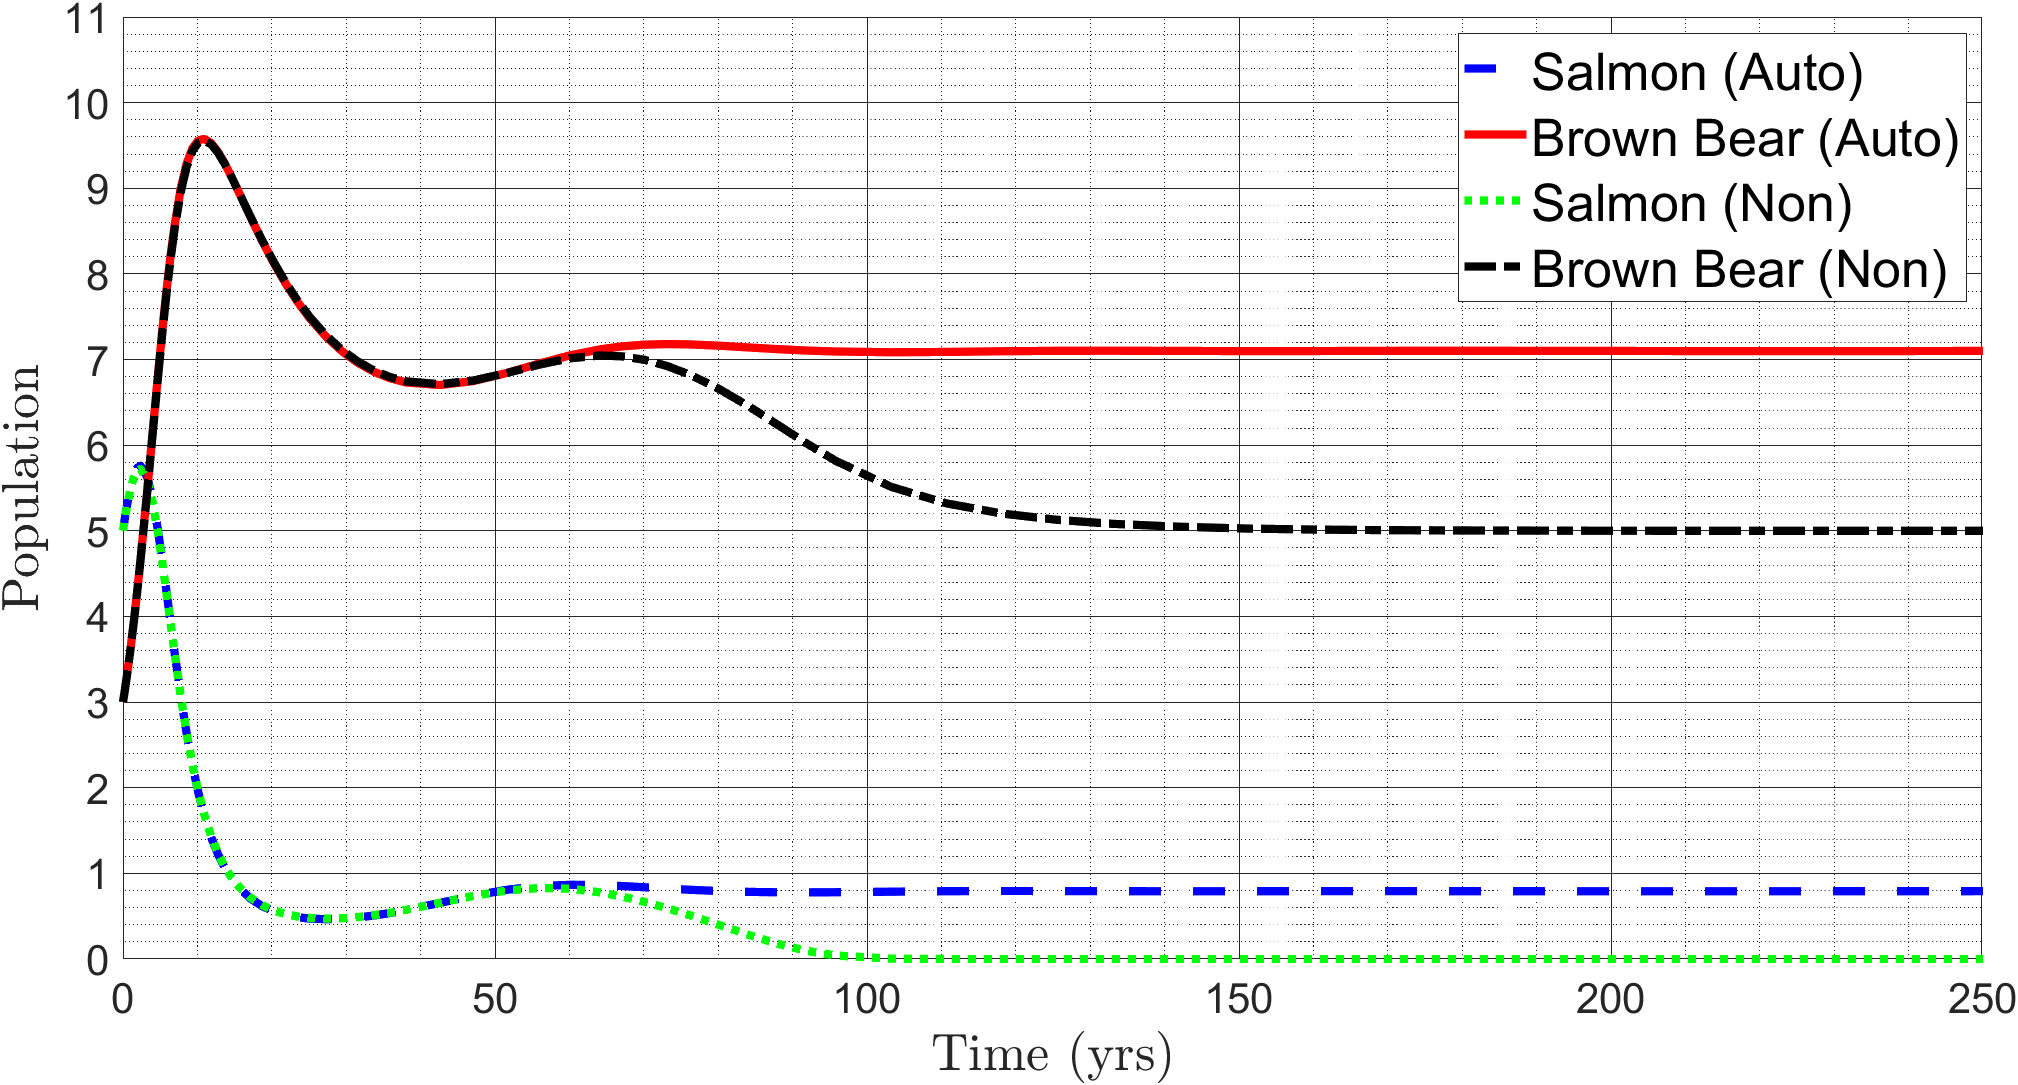
\includegraphics[width=14cm]{Pictures/System ODEs/AutonomousVsNonautonomous.png}
    \caption{\singlespacing
    Plot of the solutions to the autonomous and non-autonomous model with respect to time.}
    \label{fig:AutonomousVsNon-Autonomous}
\end{figure}
Initially, the two models follow the same path, but after approximately 60 years, the curves begin to deviate.
According to our temperature function, \equationautorefname~\eqref{eq:sstmodel}, the projected Alaskan river temperature in 60 years is $T(60)\approx14.34^{\circ}$C.
Therefore, the graph illustrates that soon after the river temperature leaves the optimal range, the difference in the outcomes of the species' populations becomes prominent.
The non-autonomous model shows similar trends to the autonomous model, but ultimately resulting in the salmon population dying off and the Alaskan brown bear population converging to its carrying capacity.










